% Template for PLoS
% Version 1.0 January 2009
%
% To compile to pdf, run:
% latex plos.template
% bibtex plos.template
% latex plos.template
% latex plos.template
% dvipdf plos.template

\documentclass[10pt]{article}

% amsmath package, useful for mathematical formulas
\usepackage{amsmath}
% amssymb package, useful for mathematical symbols
\usepackage{amssymb}

% graphicx package, useful for including eps and pdf graphics
% include graphics with the command %\includegraphics
\usepackage{graphicx}

% cite package, to clean up citations in the main text. Do not remove.
\usepackage{cite}

\usepackage{color} 

% Use doublespacing - comment out for single spacing
%\usepackage{setspace} 
%\doublespacing


% Text layout
\topmargin 0.0cm
\oddsidemargin 0.5cm
\evensidemargin 0.5cm
\textwidth 16cm 
\textheight 21cm

% Bold the 'Figure #' in the caption and separate it with a period
% Captions will be left justified
\usepackage[labelfont=bf,labelsep=period,justification=raggedright]{caption}

% Use the PLoS provided bibtex style
\bibliographystyle{plos2009}

% Remove brackets from numbering in List of References
\makeatletter
\renewcommand{\@biblabel}[1]{\quad#1.}
\makeatother


% Leave date blank
\date{}

\pagestyle{myheadings}
%% ** EDIT HERE **


%% ** EDIT HERE **
%% PLEASE INCLUDE ALL MACROS BELOW

%% END MACROS SECTION

\begin{document}

% Title must be 150 characters or less
\begin{flushleft}
{\Large
\textbf{In silico identification and in vivo validation of anti-psychotic drug fluspirilene as a potential CDK2 inhibitor and a candidate anti-cancer drug}
}
% Insert Author names, affiliations and corresponding author email.
\\
Xi-Nan Shi$^{1,3}$,
Hongjian Li$^{2}$,
Xu Liu$^{1}$,
Ling Li$^{1}$,
Kwong-Sak Leung$^{2}$,
Man-Hon Wong$^{2}$,
Hsiang-fu Kung$^{1}$,
Marie Chia-mi Lin$^{1,4,\ast}$
\\
\bf{1} Biotechnology Center, Kunming Medical University, Kunming, Yunnan, China
\bf{2} Department of Computer Science and Engineering, Chinese University of Hong Kong, Shatin, New Territories, Hong Kong
\bf{3} Department of Medicine, Southwest Guizhou Vocational and Technical College for Nationalities, Guizhou, China
\bf{4} Shenzhen Key Lab of Translational Medicine of Tumor, School of Medicine, Shenzhen University, Shenzhen, China
\\
$\ast$ E-mail: mcmlin@163.com
\end{flushleft}

% Please keep the abstract between 250 and 300 words
\section*{Abstract}
Human colorectal cancer has been reported to express high level of cyclin-dependent kinase 2 (CDK2), a key factor regulating the cell cycle G1 to S transition and a hallmark for cancers. In this study, we used idock prospectively for the first time to identify potential CDK2 inhibitors from 4,311 FDA-approved small molecule drugs with a repurposing strategy. Among the top compounds sorted by idock score, nine were purchased. Among them, adapalene (CD271,6-[3-(1-adamantyl)-4-methoxyphenyl]-2-naphtoic acid) exhibited the highest anti-proliferative effect in human colon cancer LOVO and DLD1 cells. We demonstrated for the first time that adapalene treatment significantly increased the percentage of cells in G1 phase, and decreased the expressions of CDK2, cyclin E and Rb, as well as the phosphorylations of CDK2 on Thr160 and Rb on Ser795. We then examined the anti-cancer effect of adapalene \textit{in vivo} in BALB/C nude mice subcutaneously xenografted with human colorectal cancer DLD1 cells. Our results showed that oral adapalene treatment significantly (p<0.05) and dose-dependently inhibited tumor growth. Adapalene (20 mg/kg) exhibited strong anti-tumor activity, comparable to that of oxaliplatin (40 mg/kg). The combination with adapalene and oxaliplatin exhibited the highest therapeutic effect. These results suggested for the first time that adapalene is a potential CDK2 inhibitor and a candidate anti-cancer drug for the treatment of human colorectal cancer.

% Please keep the Author Summary between 150 and 200 words
% Use first person. PLoS ONE authors please skip this step. 
% Author Summary not valid for PLoS ONE submissions.   
%\section*{Author Summary}

\section*{Introduction}
Cyclin-dependent kinase (CDK2) is one of the serine/threonine protein kinases. It plays a pivotal role in regulating the cell cycle transition from G1 to S phase, and thus in controlling cell proliferation. Abnormally high expression of CDK2 has been reported in many human neoplasias, such as colorectal, ovarian, breast and prostate cancers. Hence, CDK2 inhibitors are potential effective anti-cancer agents.

Although a number of CDK2 inhibitors have been described in the literature and some have entered clinical trial phases \cite{1603}, e.g. flavopiridol \cite{1596}, roscovitine \cite{1597} and olomoucine \cite{1598}, none of them is available for clinical use due to various reasons such as toxicity and multi-target specificity.

We utilized our free and open-source protein-ligand docking software idock \cite{1153,1362} to screen FDA-approved small molecule drugs against CDK2. We adopted the approach of structure-based virtual screening to repurpose approved toxicity-free drugs for the treatment of cancers that involve CDK2 regulation.

\section*{Methods and Materials}

\subsection*{Docking}

44 X-ray crystallographic structures of CDK2 in complex with a ligand (Table \ref{PDBs}) were collected from the PDB (Protein Data Bank) \cite{540,537}. The co-crystallized ligands and waters were manually removed. The structures of FDA-approved drugs were collected from the dbap and fda catalogs of the ZINC database \cite{532,1178}. The dbap catalog of version 2014-03-19 comprising 1,738 compounds and the fda catalog of version 2012-07-25 comprising 3,176 compounds were downloaded, of which 4,311 compounds were unique. The 44 CDK2 structures in PDB format and the 4,914 compounds in Mol2 format were then converted to PDBQT format using AutoDockTools \cite{596}. Our free and open-source docking software idock v2.1.2 \cite{1153,1362} was then executed to predict the binding conformations and the binding affinities of the 4,914 compounds when docked against the 44 CDK2 structures using an ensemble docking strategy. Finally the compounds were sorted in the ascending order of their predicted binding free energy averaged across the 44 CDK2 structures, and the top commercially available compounds were queried and purchased via http://www.chemicalbook.com/ and subsequently validated \textit{in vitro} and \textit{in vivo}.

\subsection*{Chemicals and antibodies}

The selected chemicals and the leading cancer drug oxaliplatin were purchased from Sigma-Aldrich, USA. Anti-cyclin D, B1, E, CDK2, Rb, Pho-CDK2 (Thr160), Pho-Rb (Ser795) and GAPDH were obtained from Cell Signaling Technology, Inc., Danvers, Massachusetts, USA.

\subsection*{Cell lines and cell culture}

Colorectal cancer cell lines LOVO and DLD1 were obtained from the American Type Culture Collection, Manassas, Virginia, USA. These cell lines were cultured in RPMI 1640 medium containing 10\% fetal bovine serum (FBS) (Invitrogen, Rockville, Maryland, USA) at 37$^\circ$C in 5\% CO$_2$ and 95\% humidified air.

\subsection*{Cell culture experimental conditions}

Cells were plated in 96-, 24-, or 6-well plates with 0.125\% FBS medium for 24 hours and then treated with 10\% FBS medium containing the testing compounds at various concentrations of 1, 3, 10, 30$\mu$M, and incubated for 24, 48, or 72 hours.

\subsection*{MTT assay}

Cells were plated at an initial density of 9x10\textsuperscript{3} cells/well in 96 well plates and incubated with 0.5mg/ml 3-(4,5-methylthiazol-2-yl)-2,5-diphenyl-tetrazolium bromide for 4 hours. The medium was then discarded and 200$\mu$l of formazan in dimethylsulphoxide (DMSO) was added. The absorbance was measured at 570 nm according the standard protocol. The IC50 values were calculated by Graphpad prime5.

\subsection*{Cell cycle analysis}

LOVO or DLD1 cells (4x10\textsuperscript{4}) were seeded in 24-well plates in RPMI 1640 medium containing 0.125\% FBS, and cultured for 24 hours. The cells were incubated in medium containing 10\% FBS and various doses of adapalene (1, 3, 10, 30 $\mu$M) for 12, 24, 36 hours at 37C, then fixed in ice-cold 70\% ethanol and stained with a Coulter DNA-Prep Reagents kit (Beckman Coulter, Fullerton, California, USA). Cellular DNA content of 1x10\textsuperscript{4} cells from each sample was determined with the use of an EPICS ALTRA flow cytometer (Beckman Coulter). Cell cycle phase distribution was analyzed with the ModFit LT 2.0 software (Verity Software House, Topsham, Maine, USA). All results were obtained from two separate experiments, each of which was done in triplicate.

\subsection*{Western blotting}

LOVO and DLD1 cells were plated at 6-well plates with 0.125\% FBS medium for 24 hours and then with 10\% FBS medium containing adapalene at concentration 3, 10, 30$\mu$M. Cells were harvested after 6 hours of incubation. Cells were lysed with RIPA buffer containing 1 mM PMSF and protease inhibitor cocktail at 4C for 30 minutes. After centrifugation at 13,000 rpm for 15 minutes, the supernatants were recovered and the protein concentration was measured by BCA Protein Assay Kit (Thermo). Equal amounts of cell lysates were resolved in 10\% SDS-PAGE and transferred onto nitrocellulose membranes (Sigma). After blocking, the membranes were incubated sequentially with the appropriate diluted primary and secondary antibodies. Proteins were detected by the enhanced chemiluminescence detection system (Amersham, Piscataway, New Jersey, USA). To ensure equal loading of the samples, the membranes were re-probed with an anti-GAPDH antibody (Cell Signalling Technologies).

\subsection*{Adapalene treatment \textit{in vivo} in nude mice xenografted with colorectal cancer DLD1 cells}

Female BALB/C nude mice, 4 to 5 weeks old from Vital River Laboratory Technology Co. Ltd, Peking, China, were kept under specific pathogen-free conditions and cared for in accordance with the guidelines of the laboratory animal ethics committee of Kunming Medical University. For the xenografted tumor growth assay, 1x10\textsuperscript{6}/0.2ml PBS DLD1 cells were injected subcutaneously into the right flank of the mice. Tumor size was measured every day. One week after inoculation when the tumors grew to a volume of 80 to 100 m\textsuperscript{3}, the mice were randomly divided into groups of 5 mice per group, and feeded by gavage daily for 21 days with 0.5\% CMC-NaCl containing various doses (15, 20, 65 and 100mg/kg) of adapalene and oxaliplatin (40mg/kg). The mice were then sacrificed by cervical dislocation. Tumor volume was calculated by the formula $V=ab^2/2$, where $a$ is the longest axis and $b$ is shortest axis.

\subsection*{Statistical analysis}

The results were obtained from at least three different experiments and expressed as mean ± SD. Statistical analysis was performed by Student’s t test and differences were considered to be statistically significant if p < 0.05. Statistically significant results are marked with the ※ symbol.

\section*{Results}

\subsection*{Ensemble docking results and selection of candidate inhibitors}

Totally 4,914 FDA-approved drugs were docked and ranked according to their average predicted binding affinity across 44 X-ray crystal structures of CDK2. Based on commercial availability, nine top-scoring compounds (Table \ref{Top9}) were selected and purchased for further investigations.

\begin{table}
\caption{The nine top-scoring compounds purchased and validated.}
\label{Top9}
\begin{tabular}{ccl}
\hline
ZINC ID & idock score (kcal/mol) & name\\
\hline
06716957 & -10.46 & nilotinib\\
03830332 & -10.43 & LS-194959\\
03784182 & -10.38 & adapalene\\
03830768 & -10.23 & estradiol benzoate\\
03881613 & -10.08 & nandrolone phenylpropionate\\
01542113 & -10.06 & vilazodone\\
00897240 & -10.01 & azelastine hydrochloride\\
33974796 &  -9.98 & latuda\\
01481956 &  -9.95 & paliperidone\\
\hline
\end{tabular}
\end{table}

\subsection*{Adapalene decreased cell viability of colorectal cancer LOVO and DLD1}

We first evaluated the anti-cancer effect of the nine compounds by MTT assay (Figure \ref{CellViabilityAgainstConcentration}). All the nine compounds decreased cell viability in LOVO and DLD1 cells, but had discrepant cytotoxicity at different concentrations. Among them, adapalene had the lowest IC50, i.e. 7.135$\mu$M for LOVO and 4.43$\mu$M for DLD1. In other words, adapalene exhibited the highest cytotoxicity compared to control with statistical significance (※p<0.05).

\begin{figure}
\centering
%\includegraphics[width=\linewidth]{../cdk2/CellViabilityAgainstConcentration.jpg}
\caption{Comparison of the effect of the nine compounds on the viability of LOVO and DLD1 colorectal cancer cells.}
\label{CellViabilityAgainstConcentration}
\end{figure}

Adapalene exhibited dose- and time-dependent inhibition effect on cell viability in LOVO and DLD1 cell lines compared to control (※p<0.05) (Figure \ref{CellViabilityAgainstTime}). Marked inhibition was observed at 10$\mu$M and 30$\mu$M, but no significant effect was observed at concentrations below 3$\mu$M.

\begin{figure}
\centering
%\includegraphics[width=\linewidth]{../cdk2/CellViabilityAgainstTime.jpg}
\caption{The growth inhibition effect of adapalene on LOVO and DLD1 colorectal cancer cells.}
\label{CellViabilityAgainstTime}
\end{figure}

\subsection*{Adapalene treatment arrested cell cycle in G1 phase in LOVO and DLD1 cells}

We analyzed the effect of adapalene treatment with concentrations of 3, 10, 30 $\mu$M for 6, 12, 24 hours on cell cycle profile in LOVO and DLD1 cells by flow cytometry (Figure \ref{G1Distribution}) in order to understand if adapalene inhibited CDK2 activities in colorectal cancer cells. Adapalene treatment significantly increased the percentage of cells in G1 phase compared to control (※p<0.05) in a dose- and time-dependent manner. At 30$\mu$M or 10$\mu$M concentrations, adapalene treatment continuously increased the percentage of G1 phase for 24 hours.

\begin{figure}
\centering
%\includegraphics[width=\linewidth]{../cdk2/G1Distribution.jpg}
\caption{Dose- and time-dependent effect of adapalene treatment on the percentage of cells in G1 phase.}
\label{G1Distribution}
\end{figure}

Figure \ref{CellCycleDistribution} shows the changes of cell cycle profile of G0-G1, S, and G2-M phases after 24 hours of adapalene treatment. The increase of the G1 phase was accompanied by the simultaneous decrease of S and G2-M phases.

\begin{figure}
\centering
%\includegraphics[width=\linewidth]{../cdk2/CellCycleDistribution.jpg}
\caption{Cell cycle distributions at 24 hours after adapalene treatment.}
\label{CellCycleDistribution}
\end{figure}

\subsection*{Adapalene treatment decreased the expressions of CDK2, Rb, cyclin E, pho-CDK2 and pho-Rb but not cyclin D and cyclin B1 in LOVO and DLD1 cells}

We investigated the effect of adapalene on the expressions of critical proteins involved in G1-to-S transition by western blotting in LOVO and DLD1 cells (Figure \ref{WesternBlot}). Adapalene treatment reduced the expressions of CDK2, Rb, pho-CDK2, pho-Rb and cyclin E. In contrast, the expression levels of cyclin D1 and cyclin B1 remained unchanged. These results are consistent with what are expected from a CDK2 inhibitor.

\begin{figure}
\centering
%\includegraphics[width=\linewidth]{../cdk2/WesternBlot.jpg}
\caption{Effect of adapalene treatment on the expressions of cyclins, CDK2 and Rb.}
\label{WesternBlot}
\end{figure}

\subsection*{Daily oral adapalene treatment reduced tumor growth \textit{in vivo} in BALB/C nude mice subcutaneously xenografted with DLD1 cells}

To evaluate the effect of adapalene on the growth of colorectal carcinoma \textit{in vivo}, BALB/C nude mice were subcutaneously injected with DLD1 cells. Carcinoma volumes were measured every 3 to 4 days after tumor appearance. At day 7 after tumor inoculation, the tumor volume reached 80 to 100 mm\textsuperscript{3}, then various doses (15, 65, 100mg/kg in 0.5\% CMC-NaCl) of adapalene were administered daily for 21 days by oral gavage. Figure \ref{AdapaleneOnTumorGrowth} shows that oral adapalene treatment significantly (※p<0.05) inhibited tumor growth. At day 21 after treatment, 15 mg/kg adapalene resulted in significant reduction of tumor weight and volume compared to control (※p<0.05). Nevertheless, there is no significant difference between 15 and 65 mg/kg adapalene treatment.

\begin{figure}
\centering
%\includegraphics[width=\linewidth]{../cdk2/AdapaleneOnTumorGrowth.jpg}
\caption{Effect of oral treatment of adapalene on tumor growth \textit{in vivo} in nude mice xenografted with DLD1 cells.}
\label{AdapaleneOnTumorGrowth}
\end{figure}

In a separate experiment, we compared the efficacy of adapalene (20mg/kg), oxaliplatin (40mg/kg) and the combination of adapalene (20mg/kg) plus oxaliplatin (40mg/kg) (Figure \ref{AdapaleneOxaliplatinOnTumorGrowth}). The anti-tumor activity of oral adapalene (20 mg/kg) was comparable to that of oxaliplatin (40 mg/kg). Importantly, the combinatorial therapy exhibited the highest therapeutic effect. These results suggested for the first time that adapalene is a potential CDK2 inhibitor and a candidate anti-cancer drug for the treatment of human colorectal cancer.

\begin{figure}
\centering
%\includegraphics[width=\linewidth]{../cdk2/AdapaleneOxaliplatinOnTumorGrowth.jpg}
\caption{Effect of oral treatment of adapalene combined with oxaliplatin on tumor growth \textit{in vivo} in nude mice xenografted with DLD1 cells.}
\label{AdapaleneOxaliplatinOnTumorGrowth}
\end{figure}

\subsection*{Structural analysis of the predicted conformation of adapalene docked against CDK2}

Figure \ref{1GZ8-ZINC03784182-ms} plots the predicted conformation of adapalene in complex with CDK2 using iview \cite{1366}. Figure \ref{1GZ8-ZINC03784182-pv} plots the intermolecular interaction diagram using PoseView \cite{748}. Adapalene was predicted to reside in the ATP-binding site of CDK2 and interact with CDK2 mainly through hydrophobic contacts with Phe82, Ile10, Leu134, Lys33 and His84, and a hydrogen bond with Lys33.

\begin{figure}
\centering
%\includegraphics[width=\linewidth]{../cdk2/1GZ8-ZINC03784182-ms.png}
\caption{The predicted conformation of adapalene in complex with CDK2.}
\label{1GZ8-ZINC03784182-ms}
\end{figure}

\begin{figure}
\centering
%\includegraphics[width=\linewidth]{../cdk2/1GZ8-ZINC03784182-pv.pdf}
\caption{The putative interactions of adapalene with CDK2.}
\label{1GZ8-ZINC03784182-pv}
\end{figure}

\section*{Discussion}

Cell cycle progress is sequentially and strictly processed through the interactions of CDKs and cyclins. Different cyclin-CDK complexes are activated in different phases of the cell cycle. When the cell cycle goes through G1 to S phase, the cyclin D1-CDK4/6 and cyclin E-CDK2 complexes are ordinally activated and the retinoblastoma protein (pRB) is hyper-phosphorylated on serine and threonine residues. The hyper-phosphorylated pRB promotes the release of E2F transcription factors, which in turn facilitate the transcription of numerous genes required for G1 to S transition and S phase progression. From the medicinal perspective, CDK2 has long been a classical and important target for cancer therapy.

Though a number of CDK2 inhibitors have entered clinical trial phases, none has been officially approved for clinical use, probably because of their toxicity and multi-target specificity. Given the obstacle that developing a new drug \textit{de novo} is a laborious and costly endeavor, repurposing toxicity-free old drugs for new uses is a favorable strategy.

The powerful synergy of \textit{in silico} methods in drug repurposing by structure-based virtual screening (SBVS) was highlighted in several recent reports \cite{1384}. To name a few successful repurposing cases by SBVS, \cite{1507} rediscovered 2,4-Dichlorophenoxy acetic acid, a well-known plant auxin, as a new anti-inflammatory agent through \textit{in silico} molecular modeling and docking studies along with drug formulation and \textit{in vivo} anti-inflammatory inspection; \cite{1506} attempted to repurpose FDA-approved drugs by an integrated SBVS approach and reported the discovery of piperacillin \textbf{1} as an inhibitor of NEDD8-activating enzyme (NAE) in cell-free and cell-based systems with high selectivity.

In addition to SBVS, ligand-based virtual screening (LBVS) also finds its successful applications in repurposing. \cite{1504} used Ultrafast Shape Recognition (USR) \cite{1379} to search for compounds with similar shape to a previously reported inhibitor of protein arginine deiminase type 4 (PAD4), a new therapeutic target for the treatment of rheumatoid arthritis, and identified a novel compound that has a strikingly different structure from the template inhibitor yet showed significant inhibition on the enzymatic activity of PAD4.

Encouraged by these successful stories, in this study we adopted the repurposing strategy, and utilized the computational methodology of SBVS by protein-ligand docking to shortlist candidates from FDA-approved small molecule drugs. Specifically, we used our fast docking program idock \cite{1153,1362} in combination with our convenient visualizer iview \cite{1366} for the task of rediscovering existing drugs as CDK2 inhibitors. idock is an exciting development not only because it has been vigorously shown \cite{1362} to outperform the state-of-the-art docking software AutoDock Vina \cite{595} in terms of docking speed by at least 8.69 times and at most 37.51 times while maintaining comparable redocking success rates, but also because it is free and open source under a permissive license. The latter guarantees that users from both industry and academia can freely utilize idock in their own projects that require protein-ligand docking.

To facilitate the use of idock, its input arguments and output results were purposely designed to be similar to those of AutoDock Vina, therefore existing users can easily transit to idock and benefit from considerable speedup in SBVS performance. Moreover, to promote prospective SBVS by idock, a web server called istar \cite{1362} was developed and made available at http://istar.cse.cuhk.edu.hk/idock, where there are as many as over 23 million purchasable small molecule compounds ready for docking against any protein supplied by the user. Both idock \cite{1153} and istar \cite{1362} would hopefully supplement the efforts of medicinal chemists in drug discovery research.

Regarding the structural data in use, there are so far as many as 347 solved X-ray crystal structures of CDK2 with a UniProt ID of P24941. To account for their structural variability and to mine knowledge from multiple structures of CDK2, we selected 44 holo structures of CDK2 in a bound state with a ligand in complex to carry out ensemble docking. The final score used to prioritize compounds was purposely designed to be the average score of that compound when docked to the 44 selected structures of CDK2 with their native ligand removed manually before docking. In this way the top-scoring compounds would guarantee a consistent binding strength on average. In the aspect of data source of approved drugs, although we chose the dbap and fda catalogs of the ZINC database \cite{532,1178}, it is also possible to use some other freely accessible drug databases such as DrugBank \cite{1594}, KEGG DRUG \cite{1595} and e-Drug 3D \cite{1125}.

After ensemble docking experiments with idock \cite{1153,1362} followed by careful visual inspections with iview \cite{1366}, we purchased nine top-ranking compounds for subsequent wet experiments. Among them, adapalene was selected for further investigations because its IC50 was less than 10 umol/L as determined by MTT assay. Adapalene is the third generation of synthetic retinoids, currently used for the topical therapy of acne vulgaris \cite{1599}. Its anti-proliferative and proapoptotic effects \textit{in vitro} were first reported in colon carcinoma cell lines (CC-531, HT-29 and LOVO) \cite{1600} and hepatoma cells (HepG2 and Hep1B) \cite{1601} by increasing the activity of caspase 3 via up-regulating bax and down-regulating bcl-2.

In this study, we reported for the first time that adapalene is a potential CDK2 inhibitor, and demonstrated for the first time that oral administration of adapalene (20 mg/kg) exhibited significant and strong anti-cancer efficacy as compared to the leading cancer drug oxaliplatin (40 mg/kg) \textit{in vivo} in nude mice xenografted with colorectal DLD1 cells. Most importantly, the combination of effective dose of adapalene and oxaliplatin produced even higher therapeutic effect, indicating that adapalene may work through a different mechanism than oxaliplatin, which further indicates that adapalene could be combined with other chemotherapy drugs to achieve synergistic therapeutic effect.

No obvious toxicity was previously reported by either intraperitoneal injection of 100 mg/kg adapalene in carrageenan induced paw oedema rat, or topic use of 10\% (10 mg/ml) in UV induced erythema guinea pig \cite{1604}. In this study, we did not observe significant change in body weight by oral administration of adapalene (15 to 100 mg/kg) for 21 days, suggesting that oral or intraperitoneal injection of adapalene is relatively safe. Intraperitoneal injection of 5 and 10 mg/kg oxaliplatin in B6D2F mice subcutaneously xenografted with colon 38 was previously reported to significantly reduced tumor weight to 38\% and 16\% of the control level, respectively, at 21 day post-treatment \cite{1605}. In this study, we tested oral oxaliplatin treatment by gavage at doses of 10, 20, and 40mg/kg, and found that 40mg/kg effectively reduced the tumor weight to 28\% of the control on day 21 post-treatment without showing any body weight change, indicating that oral administration of oxaliplatin is relative safe and effective.

\section*{Conclusions}

This study presents the first successful prospective application of idock \cite{1153,1362} in identifying CDK2 inhibitors from FDA-approved small molecule drugs using a repurposing strategy. We showed that adapalene (CD271,6-[3-(1-adamantyl)-4-methoxyphenyl]-2-naphtoic acid), currently used for the topical therapy of acne vulgaris, exhibited anti-cancer effect in human colorectal LOVO and DLD1 cells. We demonstrated for the first time that oral adapalene treatment significantly and dose-dependently inhibited tumor growth. Most importantly, the combinatorial therapy of adapalene and the leading cancer drug oxaliplatin exhibited higher therapeutic effect. These results suggested for the first time that adapalene is a potential CDK2 inhibitor and a candidate anti-cancer drug for the treatment of human colorectal cancer. The potential application of adapalene combined with other chemotherapy drugs for the treatment of colorectal neoplasms and other cancers warrants further investigations.

% Do NOT remove this, even if you are not including acknowledgments
\section*{Acknowledgements}

%\section*{References}
% The bibtex filename
\bibliography{refworks}

\section*{Figure Legends}

\begin{figure}[!ht]
\begin{center}
%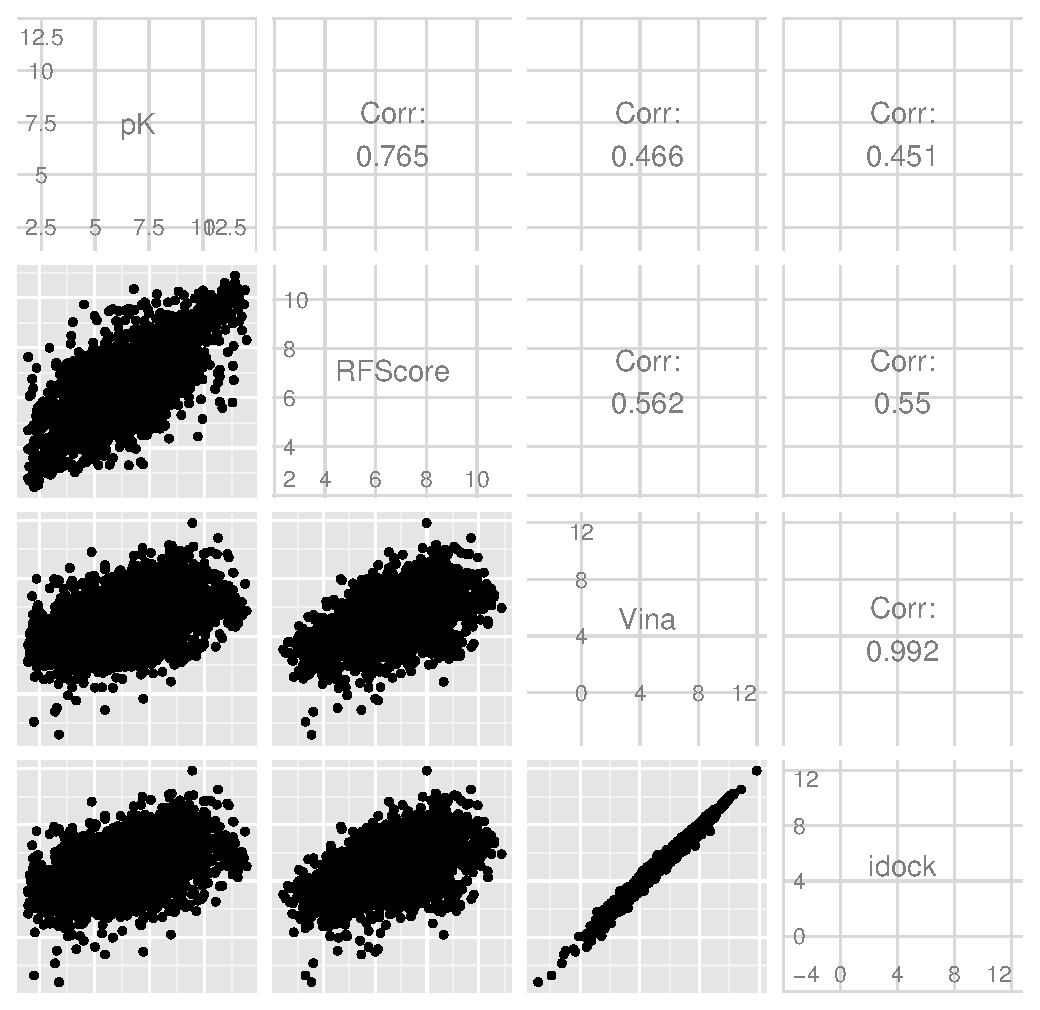
\includegraphics[width=4in]{../istar/PDBbind2012Correlations.eps}
\end{center}
\caption{
{\bf Pairwise correlations of experimental binding affinity and predicted binding affinity by RF-Score, AutoDock Vina and idock on the PDBbind v2012 refined set ($N$ = 2,897).} Values are in $pK_d$ or $pK_i$ unit. The three scoring functions are all trained on the PDBbind v2007 refined set ($N$ = 1,300). $R_p$ = 0.765, $R_s$ = 0.755, $RMSE$ = 1.26, $SD$ = 1.26 for RF-Score, $R_p$ = 0.466, $R_s$ = 0.464, $RMSE$ = 1.74, $SD$ = 1.74 for Vina, and $R_p$ = 0.451, $R_s$ = 0.453, $RMSE$ = 1.75, $SD$ = 1.75 for idock.
}
\label{PDBbind2012Correlations}
\end{figure}

\section*{Tables}

\begin{table}[!ht]
\caption{
\bf{The 44 CDK2 holo structures used for ensemble docking.}}
\begin{tabular}{ccc}
\hline
PDB ID & Resolution (\AA) & UniProt ID\\
\hline
1AQ1 & 2.00 & P24941\\
1CKP & 2.05 & P24941\\
1DI8 & 2.20 & P24941\\
1DM2 & 2.10 & P24941\\
1E1V & 1.95 & P24941\\
1E1X & 1.85 & P24941\\
1FVT & 2.20 & P24941\\
1G5S & 2.61 & P24941\\
1GIH & 2.80 & P24941\\
1GII & 2.00 & P24941\\
1GIJ & 2.20 & P24941\\
1GZ8 & 1.30 & P24941\\
1H00 & 1.60 & P24941\\
1H01 & 1.79 & P24941\\
1H07 & 1.85 & P24941\\
1H08 & 1.80 & P24941\\
1H0V & 1.90 & P24941\\
1H0W & 2.10 & P24941\\
1JSV & 1.96 & P24941\\
1JVP & 1.53 & P24941\\
1KE5 & 2.20 & P24941\\
1KE6 & 2.00 & P24941\\
1KE7 & 2.00 & P24941\\
1KE8 & 2.00 & P24941\\
1KE9 & 2.00 & P24941\\
1OIQ & 2.31 & P24941\\
1OIR & 1.91 & P24941\\
1OIT & 1.60 & P24941\\
1P2A & 2.50 & P24941\\
1PF8 & 2.51 & P24941\\
1PXI & 1.95 & P24941\\
1PXJ & 2.30 & P24941\\
1PXK & 2.80 & P24941\\
1PXL & 2.50 & P24941\\
1PXM & 2.53 & P24941\\
1PXN & 2.50 & P24941\\
1PXO & 1.96 & P24941\\
1PXP & 2.30 & P24941\\
1PYE & 2.00 & P24941\\
1R78 & 2.00 & P24941\\
1URW & 1.60 & P24941\\
1V1K & 2.31 & P24941\\
1VYZ & 2.21 & P24941\\
1W0X & 2.20 & P24941\\
\end{tabular}
\begin{flushleft}\label{PDBs}
\end{flushleft}
\end{table}

%\section*{Supporting Informatio n Legends}

\end{document}
